\section{Model Selection}

This report proposes the use of three families of models, \textit{\( k \)-Nearest neighbours, Decision trees and Logistic Regression}, in predicting the presence of disease through clinical measures. For each family of model, a range of hyperparameters are validated via \( 5 \)-fold cross-validation to choose the best candidate. Sensitivity (or True positive rate / TPR) is used as a reference to select the best performing model, with a caution that a high TPR needs not translate to good performance but rather due to underfitting, as the `True' label would be predicted at a impractical high probability.

To ease the fine-tuning process, a default of threshold of \( \delta = 0.5 \) is maintained throughout all models.

\subsection{\( k \)-Nearest neighbours (\( k \)-NN)}

\subsubsection{Methodology.}

\( k \)-Nearest neighbours (\( k \)-NN) is a simple, distance-based machine learning classification algorithm that lazily learns its class based on the majority class (for classification) or average value (for regression) of its nearest peers.

Due to \( k \)-NN's 'distance-based' nature, categorical features cannot be directly interpreted, hence they need to be transformed to numerical vectors. As in the dataset, most of the variables are numerical or ordinal values, the data is fed into the algorithm \textit{per se}, i.e., by \textit{label encoding}.

Another factor to be concerned of is feature scaling, as different measurements are made in different scales. Two scaling methods are tested: \textit{Normalisation}, where each feature is mapped to the range \( [0, 1] \) via a min-max transformation:

\begin{align*}
    \mathbf{x} \mapsto \frac{\mathbf x - \min\mathbf x}{\max\mathbf x - \min\mathbf x}
\end{align*}

and \textit{Box-Cox + Standardisation}, where each feature is fed to a Box-Cox transformation with its according optimal parameter \( \lambda \) (if applicable), then standardised:

\begin{align*}
    \mathbf{x} 
        \mapsto \mathbf{x'} := \frac{\mathbf{x}^\lambda - 1}\lambda  
        \mapsto \frac{\mathbf x' - \overline{\mathbf x'}}{\mathrm{std\ }\mathbf x'}
\end{align*}

\subsubsection{Experiments \& Results.}

\begin{table}[h]
    \centering
    \begin{tabular}{ccc}
        \toprule
        TPR, \( 19 \)-NN
        & \textbf{Full}
        & \textbf{Simplified\footnotemark{}}
        \\
        \midrule
        \textbf{Normalisation}
        & \( 86.274\% \)    
        & \( 88.697\% \)
        \\
        \midrule
        \textbf{Box-Cox + Standardisation}
        & \( 90.184\% \)    
        & \( 93.188\% \)
        \\
        \bottomrule
    \end{tabular}
    
    \raggedright
    \( ^1 \) {\small \texttt{fbs}, \texttt{bp} and \texttt{chol} are excluded from the model}
    
    \centering
    \vspace{4pt}
    \caption{\centering TPR performance of \( k \)-NN models, where \( k = 19 \)}
\end{table}

A total of four models are tested on a various range of values for \( k \in [3, 50]\), with a label cutoff at \( \delta = 0.5 \). It is observed that the simplified model with Box-Cox transformation followed by standardisation performed the best, with \( \text{TPR} = 93.94\% \) saturated at \( k \ge 19 \). 

\begin{figure}[H]
    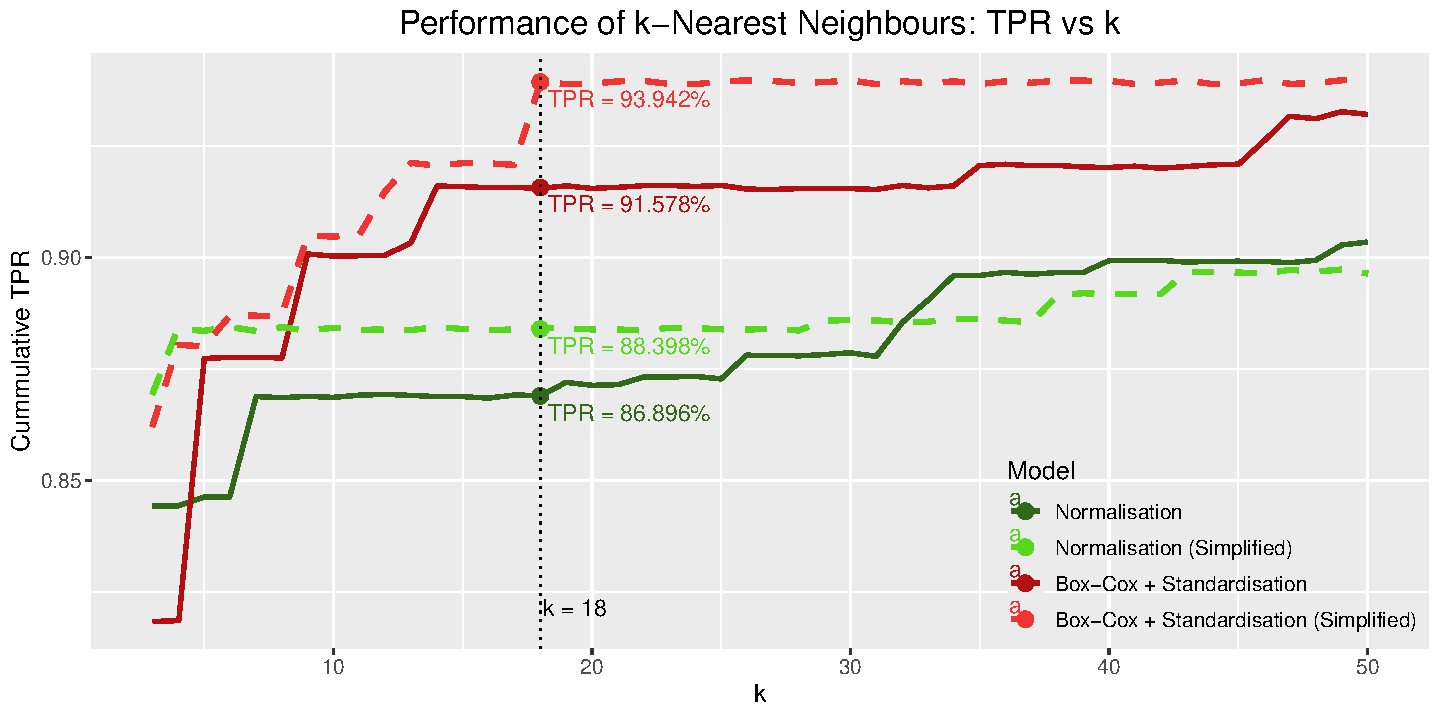
\includegraphics[width=\linewidth]{31.kNN.pdf}
    \caption{\centering TPR performance of \( k \)-NN models with running \(k\)}
\end{figure}
    
Generally, standardisation methods outperform normalsation as the best preprocessing method for \( k \)-NN. In terms of model complexity, simple models fit best for small values of \( k \), however when \( k \) gets larger, then simple models fit the data worse compared to full models; this may rather shows the effect of underfitting than outperformance. By the elbow method, it can be seen that the best performing model is a \textbf{\( 19 \)-nearest neighbour model on a Box-Cox, standardised dataset}.

\subsection{Decision tree}
\subsubsection{Methodology.}
Decision Tree is a rule-based machine learning algorithm, where its set of rules is generated by recursively splitting the dataset on a chosen feature so that the separation maximises a certain target criterion (e.g. entropy gain, Gini impurity, etc.). Despite being generally less accurate comparing to other machine learning models, it rises in terms of comprehensibility and explainability. As the algorithm does not assume the underlying distribution of the data, transformation such as standardisation or Box-Cox are not required at this stage.

\subsubsection{Experiments \& Results.}
Experiments focus in finding the best splitting algorithm, that includes the criterion to be optimised for splitting and the terminating condition. In other words, the following parameters are tested:

\begin{itemize}
    \item \textbf{\texttt{minsplit}}. Number of elements in a leaf node, where the algorithm stops splitting. \texttt{minsplit} is let to be \( 5, 10, 15, \cdots, 100 \);
    \item \textbf{\texttt{split}}. Algorithm to determine the optimal split. Either 'Information gain' (Entropy gain) or 'Gini impurity'.
\end{itemize}

In terms of sensitivity at \( \delta = 0.5 \), entropy-based algorithms fit well for a low \texttt{minsplit}, but as \texttt{minsplit} increases, its performance stagnated, both in the full or simplified tree. In contrast, Gini-based trees underperform with low values of \texttt{minsplit}, but gradually improve when \texttt{minsplit} increases. There is also an observation that simplifing the input does not change the metrics for large \texttt{minsplit}s, suggesting the possibility that the algorithm abandons these uncorrelated features at its internal procedures.

\begin{figure}[h]
    \centering
    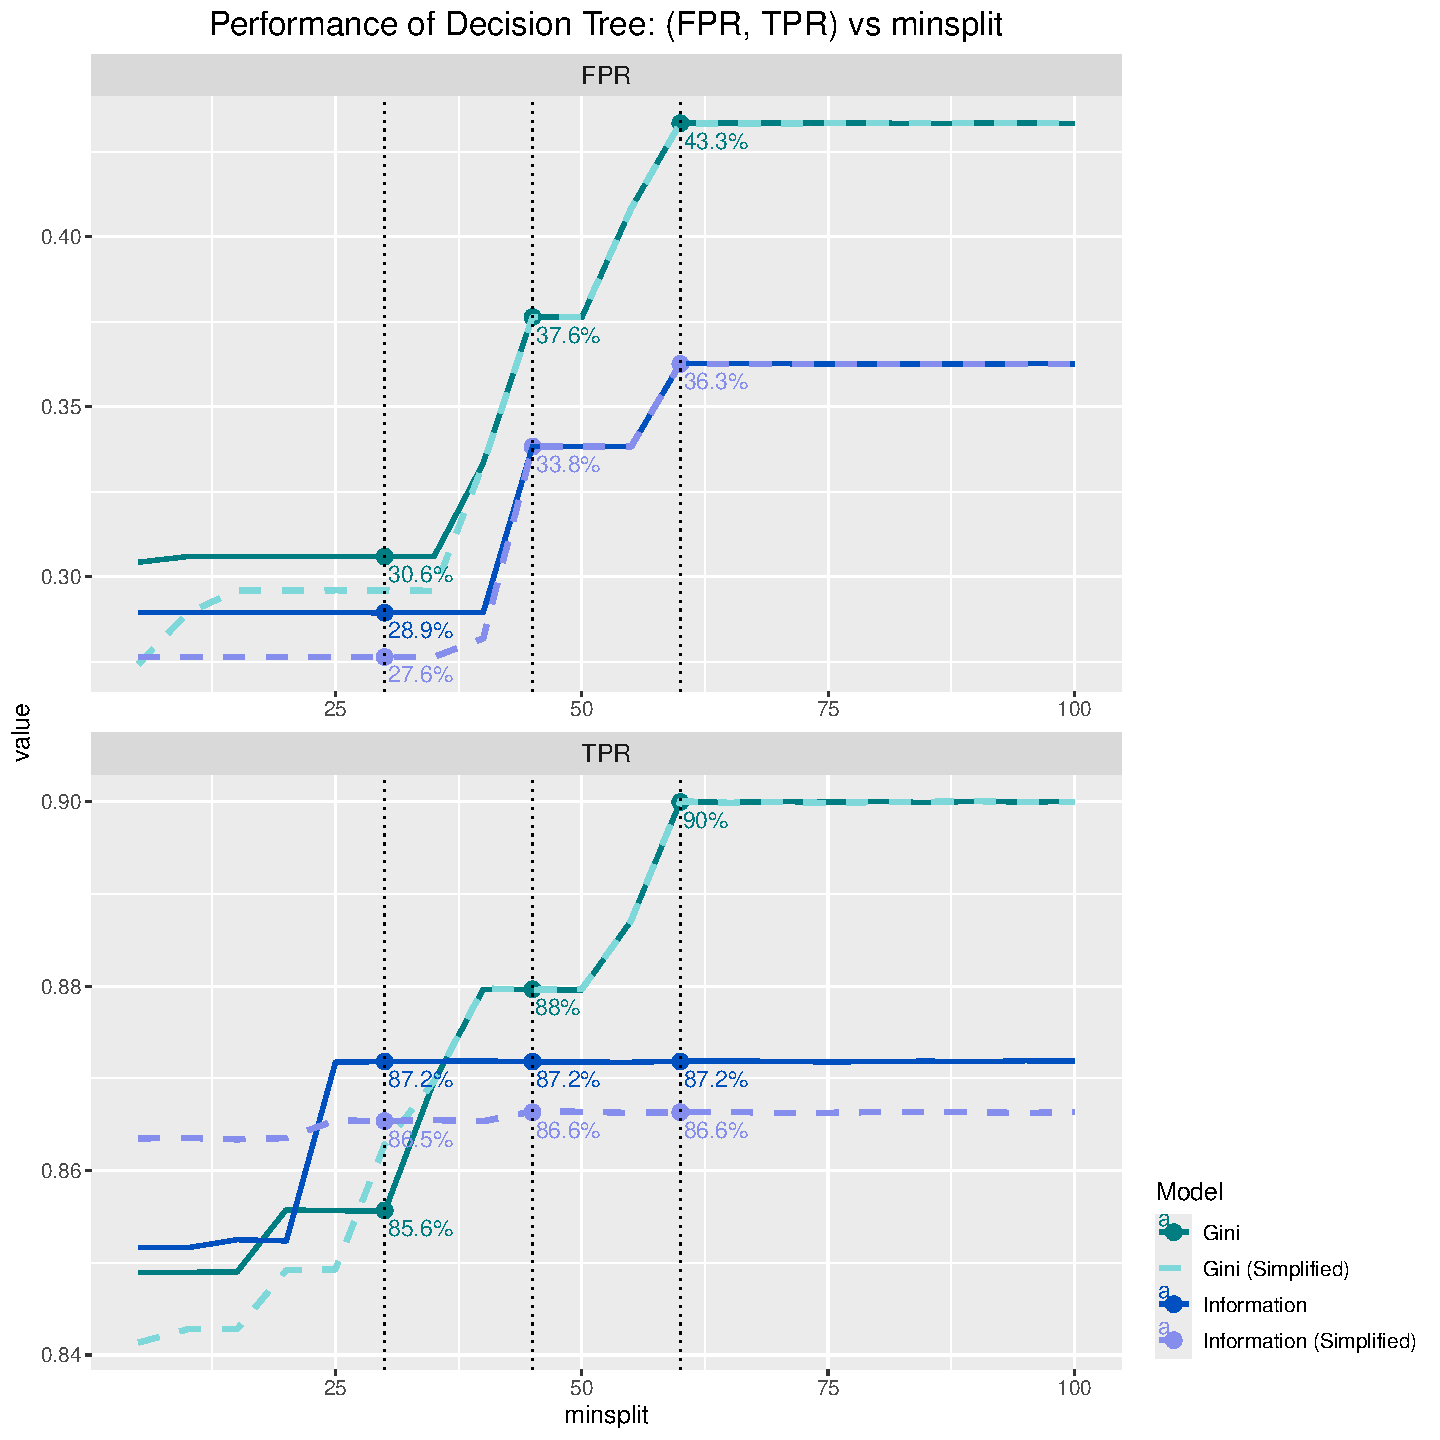
\includegraphics[width=\linewidth]{32.DecisionTree.pdf}
    \caption{\centering TPR/FPR performance of decision trees vs. minsplit}
\end{figure}

One should be cautious, however, when setting a high value of \texttt{minsplit}, as it would result in an underfitting tree with most of the datapoint classified as True, optimising TPR at the cost of a high False Positive Rate (FPR). In this example, although a decision tree with \( \texttt{minsplit} = 60 \) produces a \( 90.0\% \) sensitivity, its speficitivity is a very impractical \( 43.3\% \). The tree structure is a simple \( 2 \)-layer tree that relies only on \texttt{blood.disorder} and \texttt{chest.pain}, hence the underfitting phenomenon.

\begin{figure}[h]
    \centering
    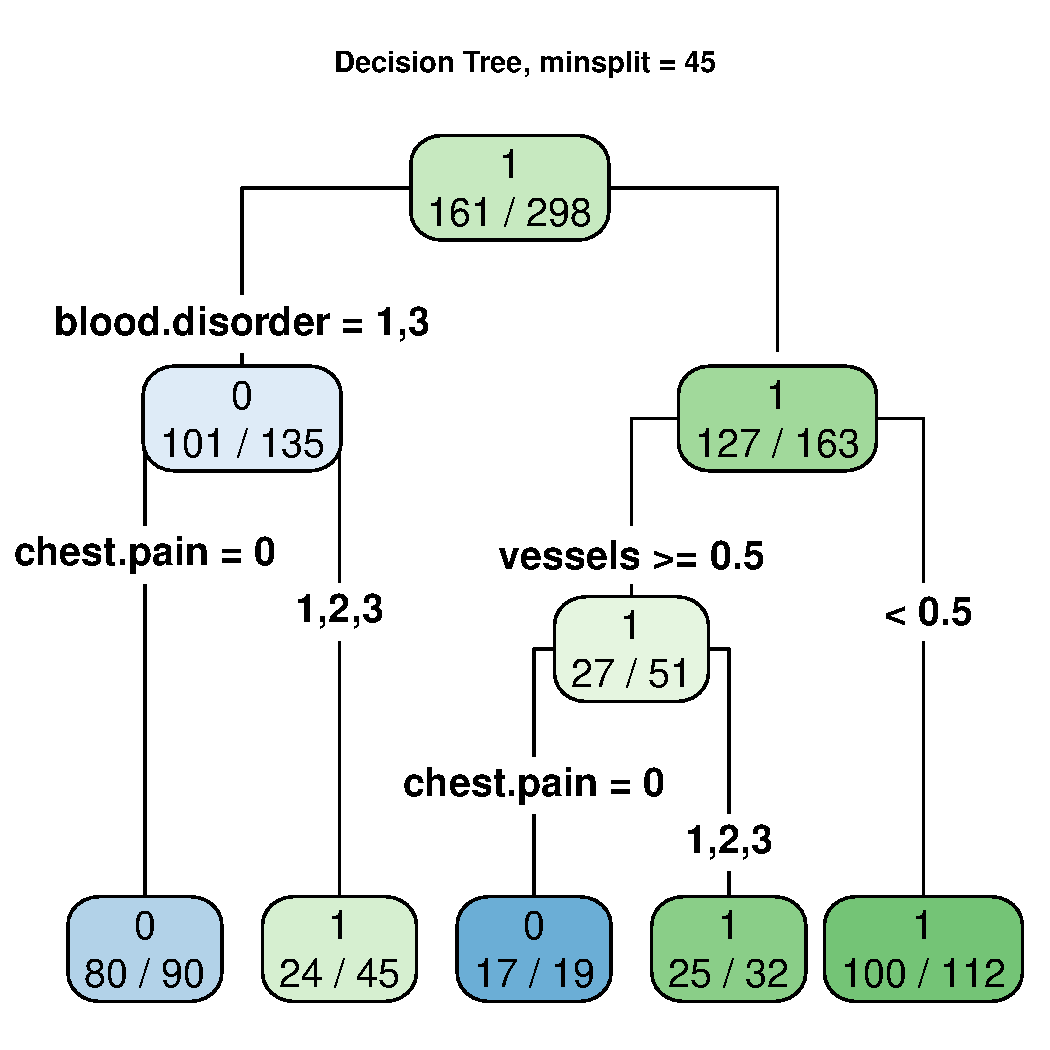
\includegraphics[width=0.45\linewidth]{32.DecisionTree-45.pdf}
    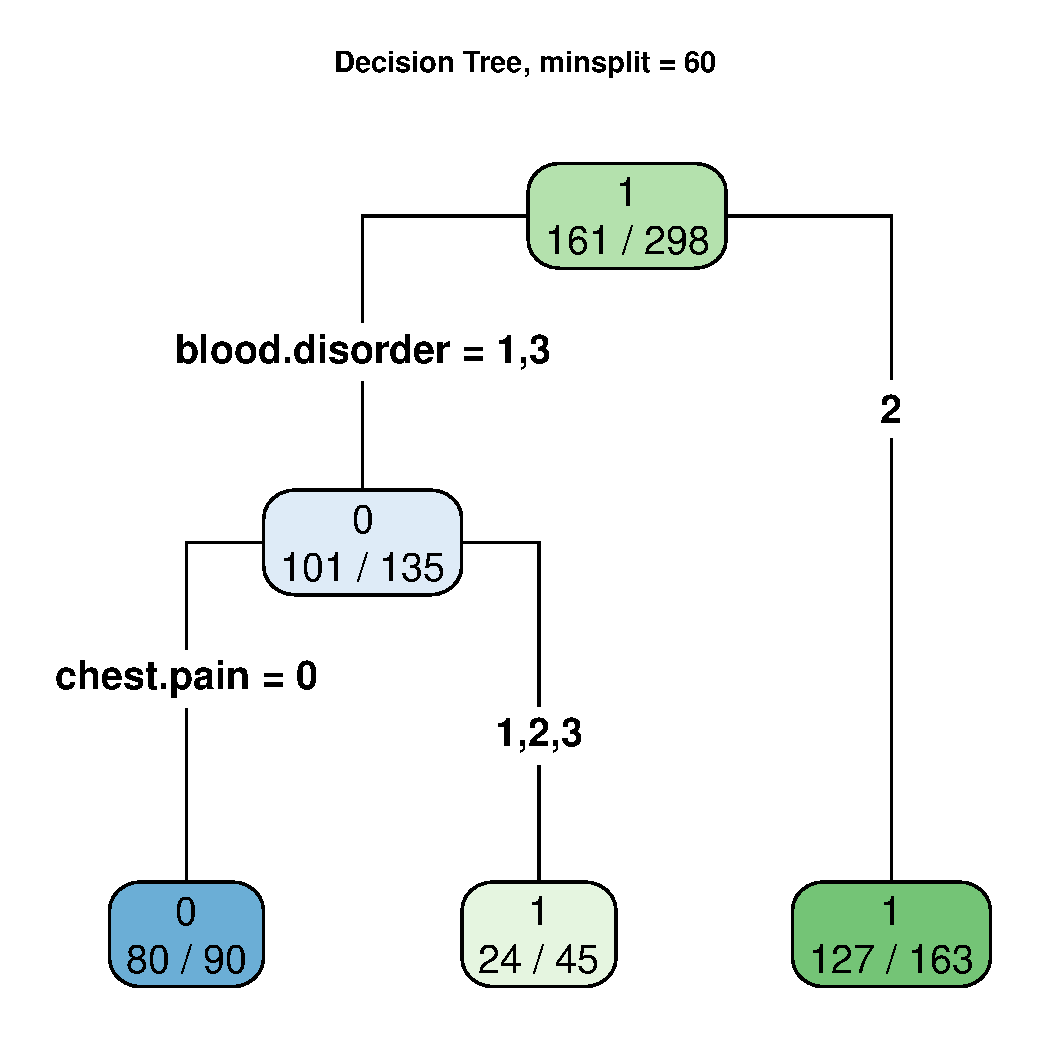
\includegraphics[width=0.45\linewidth]{32.DecisionTree-60.pdf}
    \caption{\centering Left: Moderate 45-minsplit decision tree; Right: Underfitting 60-minsplit decision tree}
\end{figure}

Choosing the 'best' model amongst all decision trees is rather a nuanced task due to the complex relationship between the \texttt{minsplit} hyperparameter with TPR-FPR metrics. For now, these two decision trees are left for further investigation:
\begin{itemize}
    \item \textbf{Information gain, \( \texttt{minsplit} = 30 \)}
    \item \textbf{Gini, \( \texttt{minsplit} = 45 \)}
\end{itemize}


\subsection{Logistic regression}


\subsubsection{Methodology}

Logistic regression is a regression model that estimates the \textit{log-odds} of an event as a linear combination of features:

\begin{align*}
    \ln \frac{\hat p}{1 - \hat p} = \hat\beta_0 + \hat\beta_1 X_1 + \cdots + \hat\beta_k X_k
\end{align*}

where \( \hat p \) is the estimator of \( \mathbb P[Y = 1] \), \( \hat\beta_0, \hat\beta_1, \cdots, \hat\beta_k \) are estimates of the linear coefficients. Unlike the usual linear regression, logistic regression has less assumption on its variable. For example, normality of independence variables is not required, hence it is not expected that logistic regression would better-fit on standardised data than the original one.

\begin{figure}[h]
    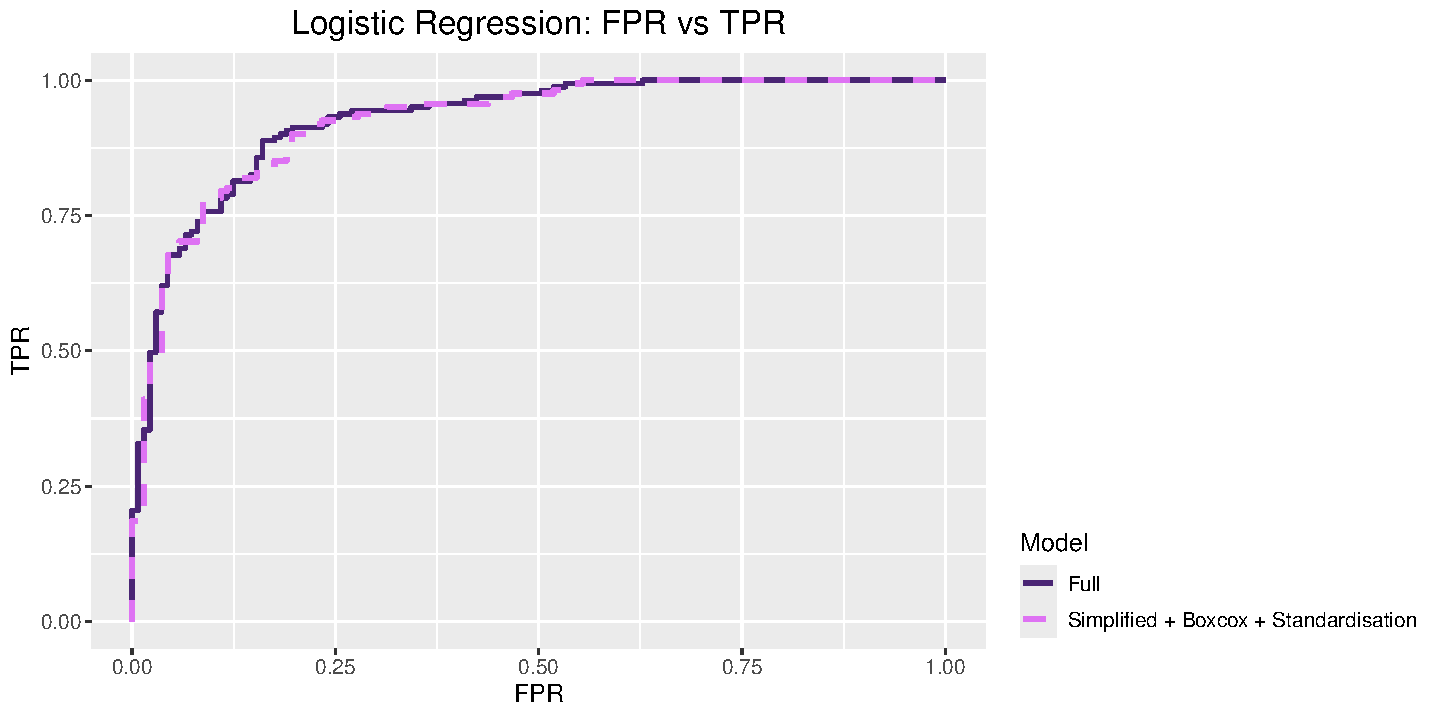
\includegraphics[width=\linewidth]{33.LogisticRegression.pdf}
    \caption{\centering ROC curve for logistic models}
\end{figure}

\subsubsection{Experiments \& Results}
Indeed, two logistic models are tested, a full model on all \( 12 \) features, and a simplified model on a Box-Cox, standardised version of only \( 9 \) significant features. They yields relatively similar results: investigation on the ROC curves produced by the two models shows that they pretty much overlap, except when \( \textrm{FPR} \approx 0.125 \) when the curve of the simplified model concaves down.

% \begin{table}[h]
%     \centering
%     \begin{tabular}{ccc}
%         \toprule
%         Logistic Regression
%             & \textbf{Full}
%             & \textbf{Box-Cox, Simplified\footnotemark{}}
%         \\
%         \midrule
%         \textbf{AUC}
%             & \( 0.9268 \)    
%             & \( 0.9235 \)
%         \\
%         \bottomrule
%     \end{tabular}
    
%     \raggedright
%     \( ^2 \) {\small \texttt{fbs}, \texttt{bp} and \texttt{chol} are excluded from the model}
    
%     \centering
%     \vspace{4pt}
%     \caption{}
% \end{table}

It can also be seen from the model coefficients that features contributing the most to the prediction of disease include \texttt{chest.pain}, \texttt{sex}, \texttt{blood.disorder} and \texttt{vessels}. There is a similarity between logistic models and decision trees, in the sense that these set of features stand as strong predictors for disease.

\begin{table}[h]
    \centering
    \begin{tabular}{lrr}
        \toprule
        \textbf{Feature} & \textbf{Estimate\footnotemark{}} & \textbf{p-value}\\
        \midrule
        \bf chest.pain3 & \bf 1.88 & \bf 0.0031\\
        \midrule
        \bf chest.pain2 & \bf 1.86 & \( \bf <  0.0001 \) \\
        \midrule
        \bf sex1 & \bf -1.31 & \bf 0.0085\\
        \midrule
        blood.disorder3 & -1.28 & 0.0954\\
        \midrule
        \bf chest.pain1 & \bf 1.11 & \bf 0.0437\\
        \midrule
        \bf vessels & \bf -0.80 & \( \bf < 0.0001 \)\\
        \midrule
        angina1 & -0.76 & 0.0716\\
        \midrule
        \bf st.depression & \bf -0.69 & \bf 0.0040\\
        \midrule
        rest.ecg1 & 0.65 & 0.0785\\
        \midrule
        \bf heart.rate & \bf 0.53 & \bf 0.0242\\
        \midrule
        (Intercept) & 0.44 & 0.6332\\
        \midrule
        rest.ecg2 & -0.30 & 0.8992\\
        \midrule
        \color{red}{chol} & 0.30 & 0.1504\\
        \midrule
        \color{red}{bp} & 0.29 & 0.1213\\
        \midrule
        blood.disorder2 & 0.21 & 0.7880\\
        \midrule
        \color{red}{fbs1} & 0.19 & 0.7367\\
        \midrule
        age & 0.01 & 0.9661\\
        \bottomrule
    \end{tabular}

    \raggedright
    \( ^\# \) {\small \textbf{bold values} indicate significant features (\( \alpha = 0.05 \))}
    
    \( ^3 \) {\small sorted by magnitude of coefficients}

    \centering
    \vspace{4pt}
    \caption{Description of the logistic model}
\end{table}

